% !TEX root = ../main.tex

\subsection{Rejection Sampling}
\label{sec:inf:foundation:rejection}

Rejection sampling is one of the simplest Monte Carlo 
inference methods and one of the only ones to produce exact samples from 
the target.  Before going into the method itself, we first consider an example to
demonstrate the underlying intuition.  Imagine we want to generate samples 
distributed uniformly over some arbitrary two dimensional shape.  One simple
way of doing this would be to sample uniformly from a box enclosing the
shape and then only taking the samples which fall 
\begin{wrapfigure}{r}{0.38\textwidth}
	\centering
	\vspace{-8pt}
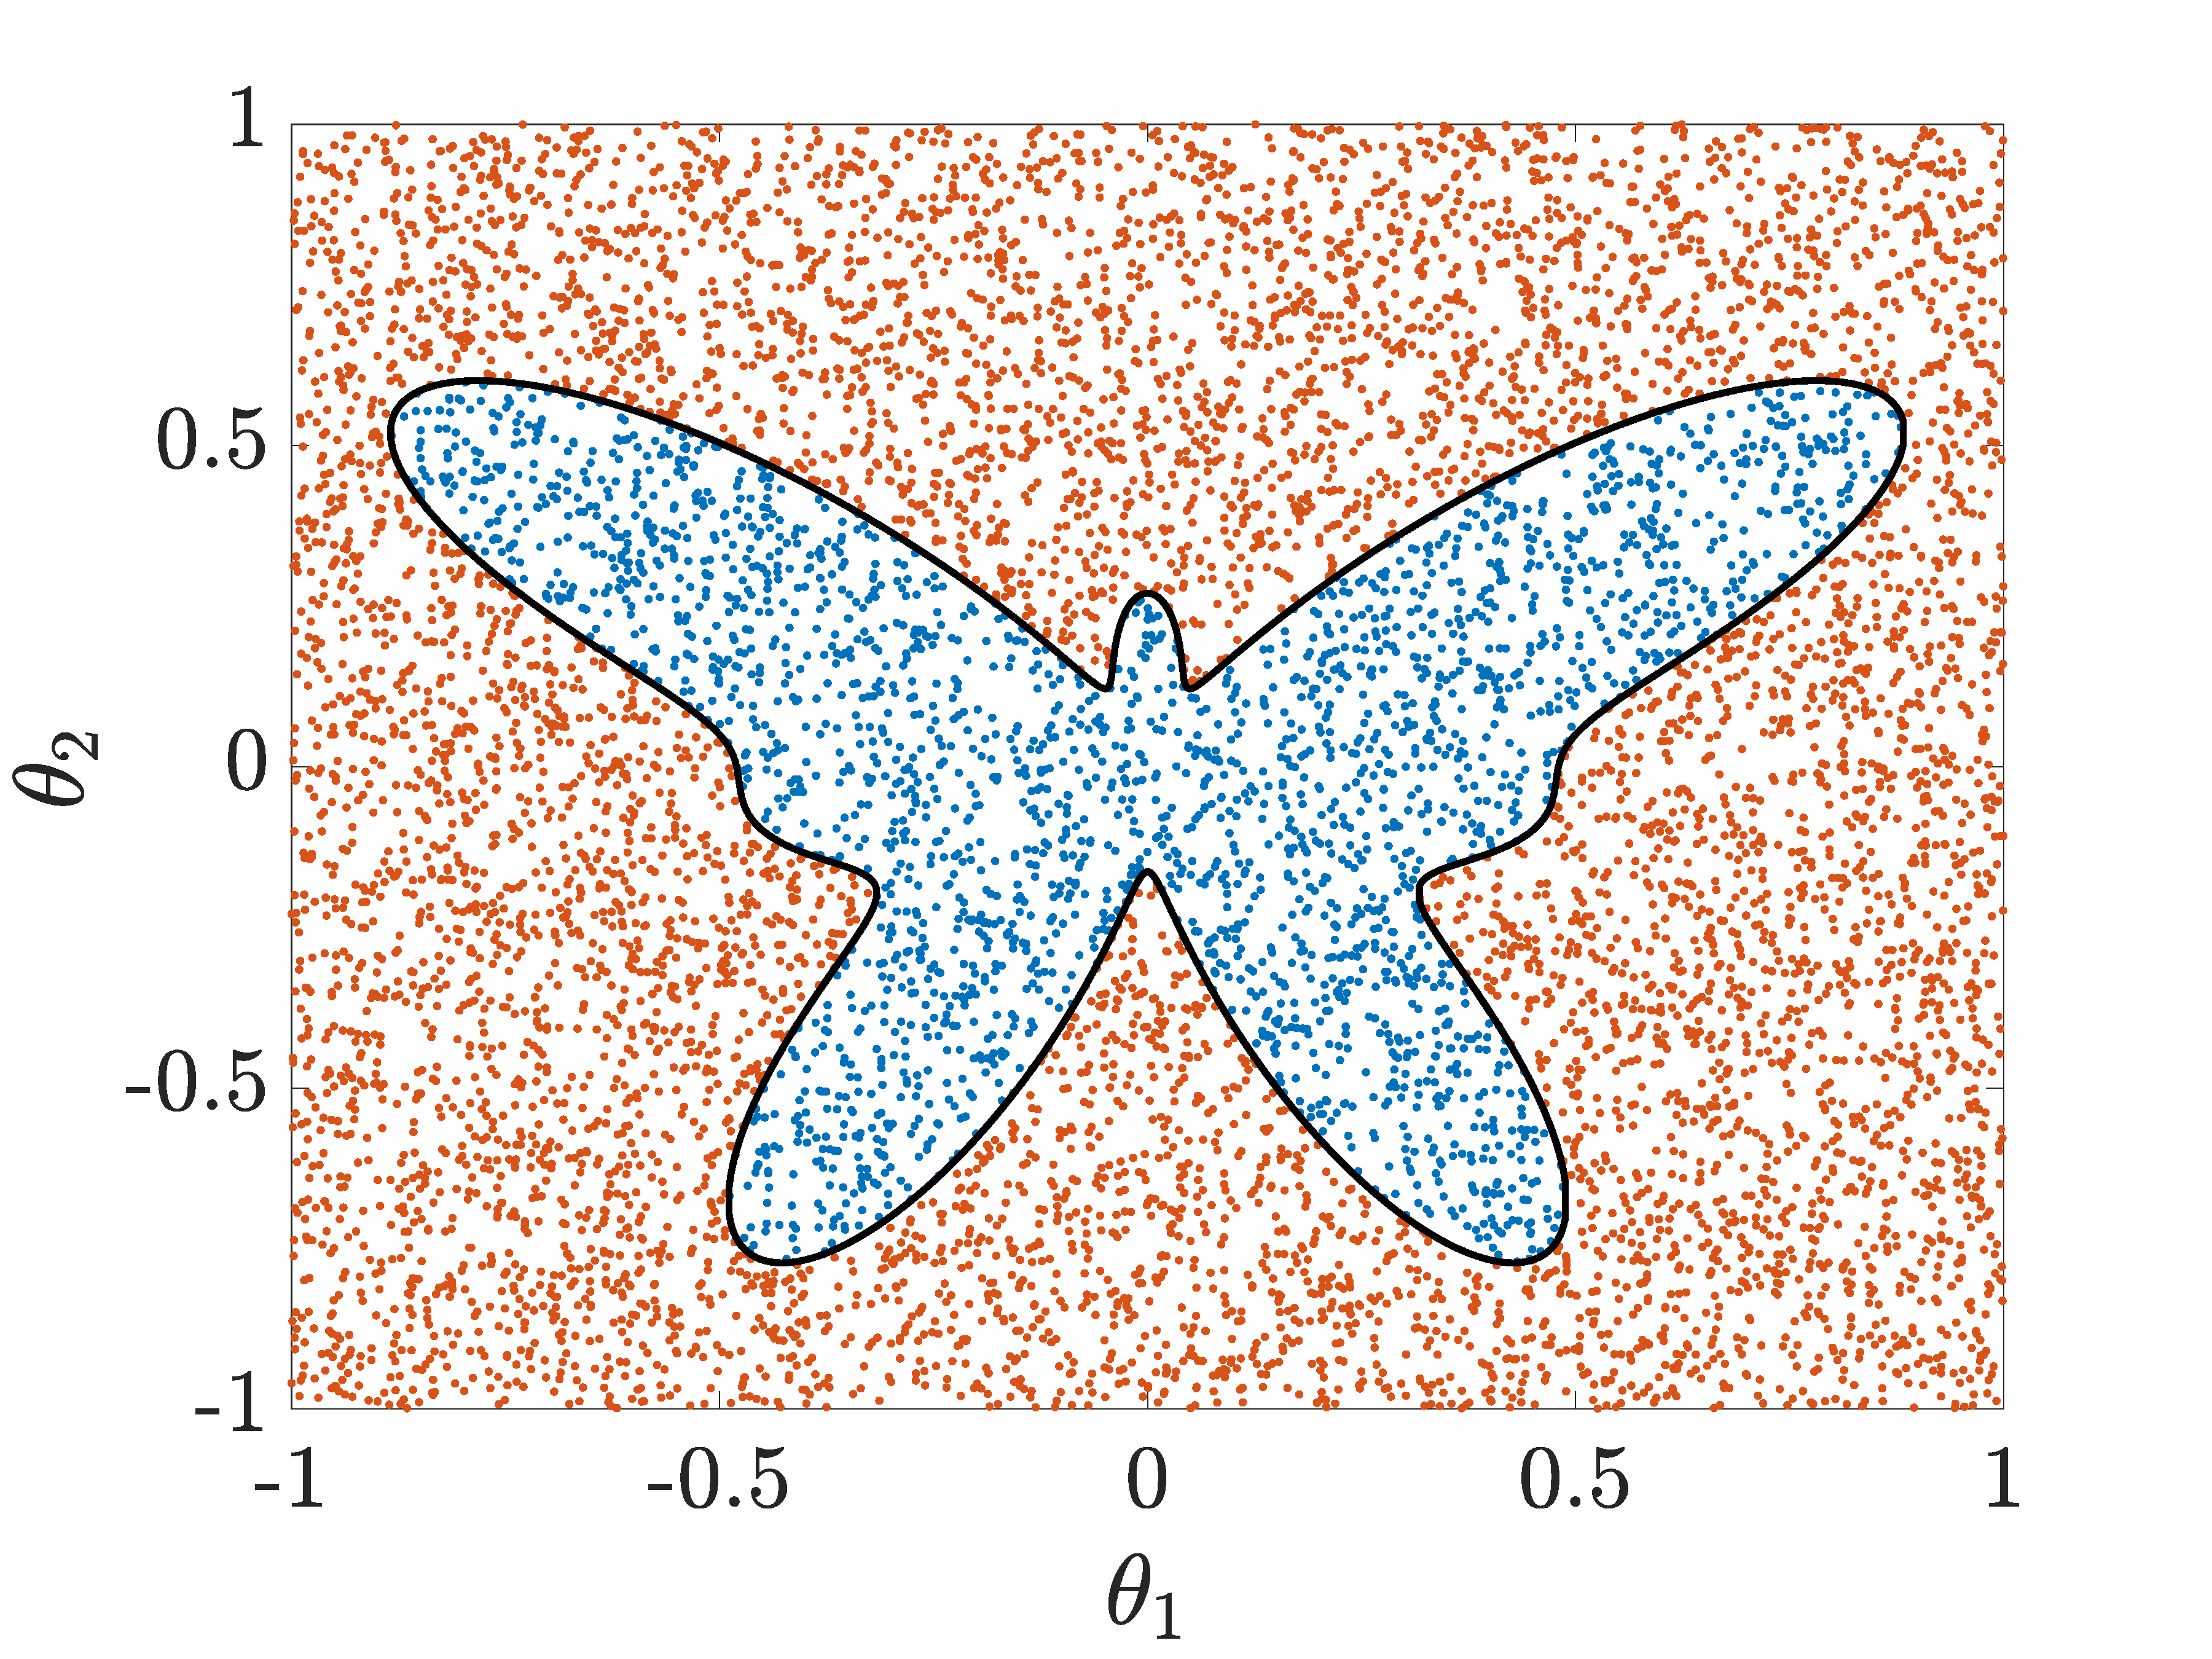
\includegraphics[width=0.37\textwidth]{butterfly}
	\vspace{-4pt}
		\caption{Sampling uniformly from an arbitrary shape by 
			rejection.  Samples are proposed uniformly from the $[-1,1]$
			square.  Any sample falling within the black outline is accepted 
			(blue), otherwise it is rejected (red).  \label{fig:inf:rej-butt}}
	\vspace{4pt}
\end{wrapfigure}
within the shape.
An example of such 
sampling by rejection is shown in Figure~\ref{fig:inf:rej-butt}.
As all the samples within the box are distributed uniformly, they are also
uniformly distributed on any subset of the space.  Therefore if we sample
from the box and then only take the samples
that fall within the desired shape, we will generated samples uniformly over
that shape. We can also use this method to estimate the area of the shape by using
the fact that the probability of any one sample falling within the shape is equal to
the ratio of the areas of the shape and the bounding box, namely
\begin{align*}
A_{\text{shape}} &= A_{\text{box}}	P(\theta \in \text{shape}) \\
&\approx \frac{A_{\mathrm{box}}}{N} \sum_{n=1}^{N} \ind (\hat{\theta}_n \in \text{shape})
\quad \text{where} \quad \hat{\theta}_n \sim \textsc{Uniform}(\text{box})
\end{align*}
where we have used a Monte Carlo estimator for $P(\theta \in \text{shape})$.
Note that the value of $P(\theta \in \text{shape})$ will
dictate the efficiency of our estimation as it represents the \emph{acceptance rate}
of our samples.  In other words, we need to generate on average $1/P(\theta \in \text{shape})$
samples from our proposal for each sample created in the target area.  As we
will show later in Section~\ref{sec:inf:foundation:curse}, $P(\theta \in \text{shape})$ typically becomes very
small as $\theta$ becomes high dimensional, so this approach will typically only
be effective in low dimensions.

The underlying idea to extend this approach to rejection sampling more generally, is that we can sample from any distribution
by sampling uniformly from the hyper-volume under its unnormalized probability density function.
Though this is effectively axiomatic by the definition of a probability density
function with respect to the Lebesgue measure, we can get a non measure-theoretic
intuition for this by considering augmenting a target distribution with a new variable $u$
such that $p(u|\theta) = \textsc{Uniform}(0,\gamma(\theta))$.  Sampling 
$\hat{\theta} \sim \pi(\theta)$ and then $\hat{u}\sim p(u|\theta)$ corresponds to
sampling uniformly from hyper-volume under the probability density function, while we
clearly have that the marginal distribution on $\theta$ is $\pi(\theta)$.

\begin{figure}[t]
	\centering
	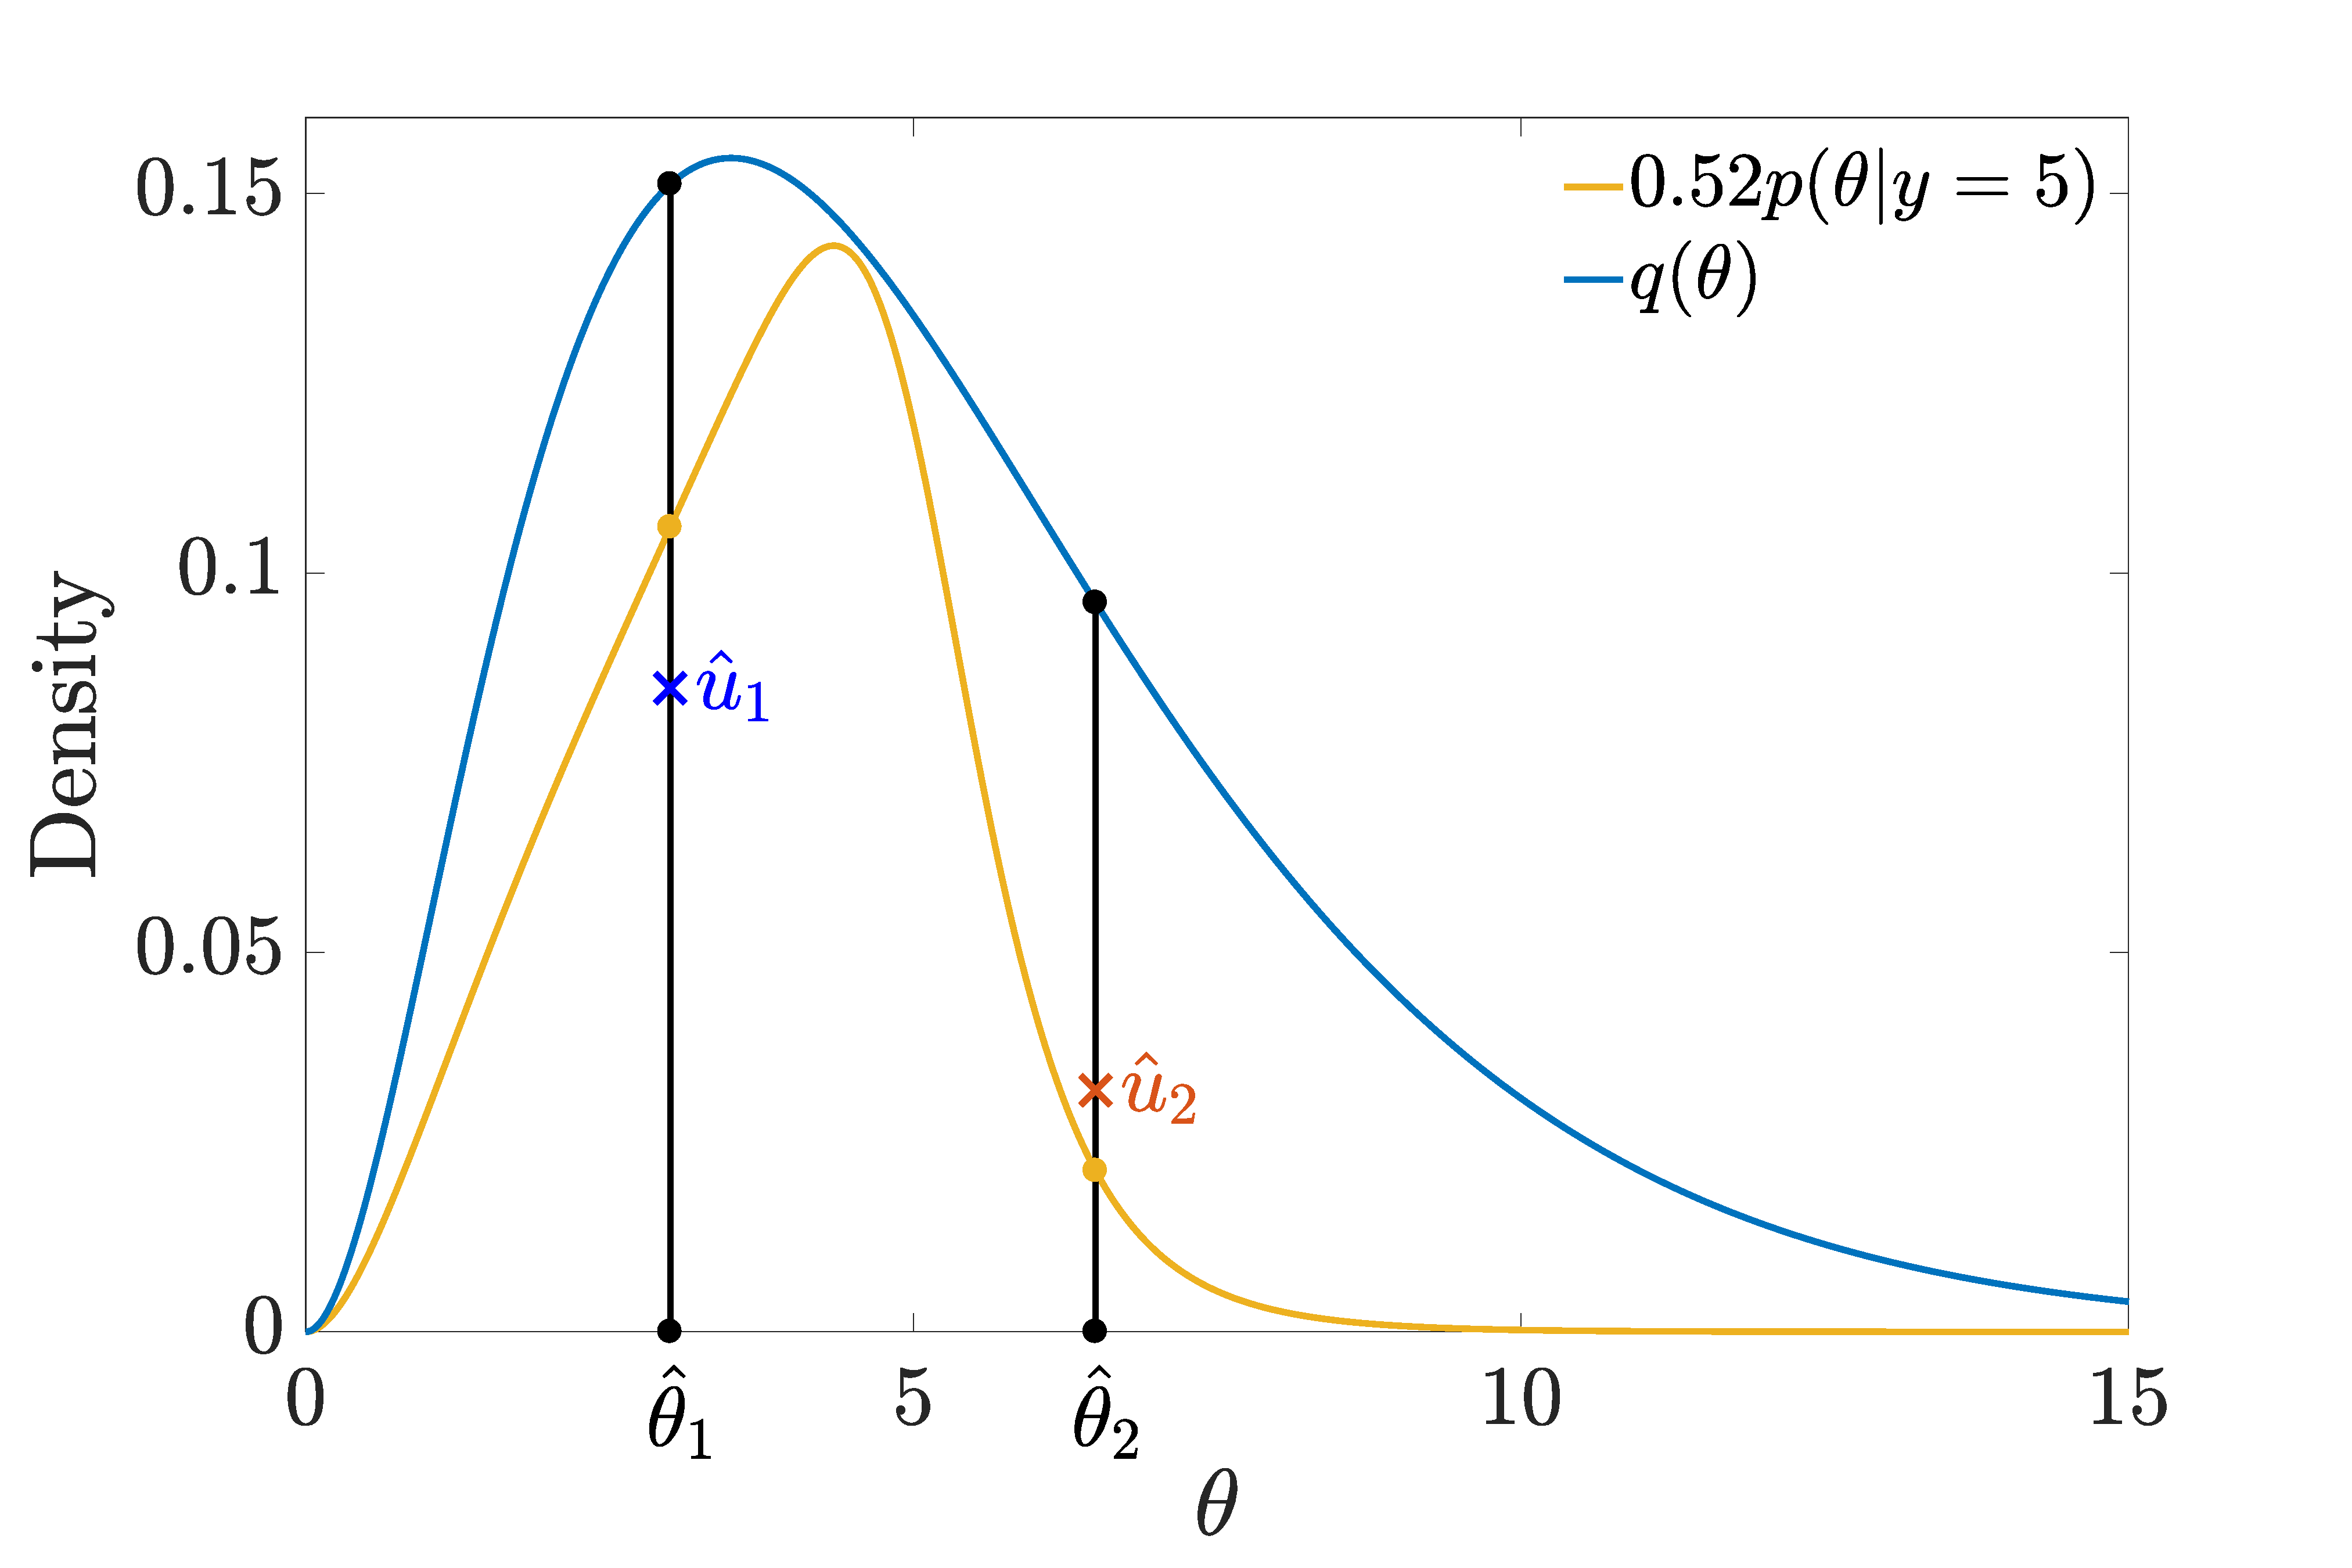
\includegraphics[width=0.6\textwidth]{reject_samp}
	\caption{Demonstration of rejection sampling for problem shown in~\eqref{eq:inf:example}.  
		We first sample $\hat{\theta}\sim q(\theta)$, correspond to the sampling for the distribution
		shown in blue,
		and then sample $\hat{u}\sim \textsc{Uniform}(0,q(\theta))$, corresponding to
		sampling a point uniformly along the black lines for the two shown example values of 
		$\hat{\theta}$.  The point is accepted 
		if $\hat{u} \le C p(\theta | y=5)$ (i.e. if it below the yellow curve) and is 
		otherwise rejected, where we have taken
		$C=0.39$ to ensure $C p(\theta | y=5)\le q(\theta)$ for all theta.
		Here the example sample pair $\{\hat{\theta}_1,\hat{u}_1\}$ is accepted, while
		$\{\hat{\theta}_2,\hat{u}_2\}$ is rejected.  The
		resulting accepted sample pairs will be uniformly sampled from the region under
		the unnormalized target distribution given by the yellow curve and therefore
		the accepted $\hat{\theta}$ will correspond to exact samples from the target.
		 \label{fig:inf:rej-samp}}
\end{figure}

Using this idea, we can sample from any unnormalized distribution by sampling from
an appropriate bounding as per Figure~\ref{fig:inf:rej-butt} and then accepting only samples
that fall within the hyper-volume of the probability density function. 
More specifically, we define a proposal
distribution $q(\theta)$ which completely envelopes a
scaled version of the unnormalized target distribution $C\gamma(\theta)$ such that 
$q(\theta)\ge C \gamma(\theta)$ for all values of $\theta$ and $C>0$.  We then sample a pair 
$\{\hat{\theta},\hat{u}\}$ by first sampling $\hat{\theta} \sim q(\theta)$ and then
$\hat{u} \sim \textsc{Uniform}(0,q(\theta))$.  The sample is accepted if
\begin{align}
	\label{eq:inf:rej-acc-criteria}
	\hat{u} \le C \gamma(\hat{\theta})
\end{align}
which occurs with an acceptance rate $CZ$ (note that $q(\theta)\ge C \gamma(\theta) \; \forall \theta$
ensures that $C \le 1/Z$).  This can be used to estimate the normalization
constant $Z$, corresponding to the marginal likelihood for Bayesian models, by calculating
the empirical estimate of the acceptance rate and dividing this by $C$.
A graphical demonstration of the rejection sampling process is shown in 
Figure~\ref{fig:inf:rej-samp}.

Rejection sampling can be a highly effective sampling or inference method in low dimensions.
In particular, the fact that it generates exact samples from the target distribution can be very
useful.  This very rare characteristic is used to construct efficient samplers for many 
common distributions such as in the ziggurat algorithm~\citep{marsaglia2000ziggurat} often
used for generating Gaussian random variables.  More generally, whenever one wishes to construct
a sampler for a non-standard low dimensional distribution, e.g. when declaring an Anglican \defdist,
rejection sampling is the clear go-to approach because it produces exact samples and because
one can usually engineer a very efficient sampler.
However, the efficiency of rejection sampling is critically dependent
on the value of $C$ because it is directly proportional to the acceptance rate.  By proxy, it
is also critically dependent on the proposal $q(\theta)$ as this dictates the minimum possible
value of $C$, namely $C_{\min} = \min_{\theta} q(\theta) Z / \pi(\theta)$.  
%Note that if 
%$q(\theta) = \pi(\theta) \; \forall \theta$ then using $C=C_{\min}$ gives an acceptance rate of $1$, while the
%more different they are (in terms of $\min_{\theta} q(\theta) / \pi(\theta)$), the lower the
%best possible acceptance rate becomes.  
%In low dimensions, adaptive rejection 
%sampling~\citep{gilks1992adaptive} often forms an effective method for adaptively 
%learning an effective proposal and corresponding value for $C$, leading to good acceptance
%rates. 
 Consequently, it is very prone to the \emph{curse of dimensionality} as
we discuss in Section~\ref{sec:inf:foundation:curse}, meaning performance cannot be
maintained for higher dimensional problems.